\section{Gemeinsam stark!}

\subsection{Raspberry Pi mit Arduino huckepack}

\begin{frame}
\frametitle{Das Problem}

Raspberry Pi ist billig und leistungsstark, aber:
\newline

\begin{itemize}
\item Viele Bibliotheken nur f�r Arduino erh�ltlich
\item Hoher Aufwand, Bibliotheken und Protokolle zu portieren
\item Keine analogen Ports
\end{itemize}
\end{frame}

\begin{frame}
\frametitle{Die L�sung}

Wir kombinieren einfach Raspberry Pi und Arduino:
\newline

\begin{center}
\textbf{Best of both worlds!}
\end{center}

\begin{itemize}
\item Alle Arduino-Bibliotheken nutzbar
\item GPIO des Raspberry bleibt erhalten
\item Weniger als 10 Euro Investition
\end{itemize}
\end{frame}

\begin{frame}
  \begin{center}
    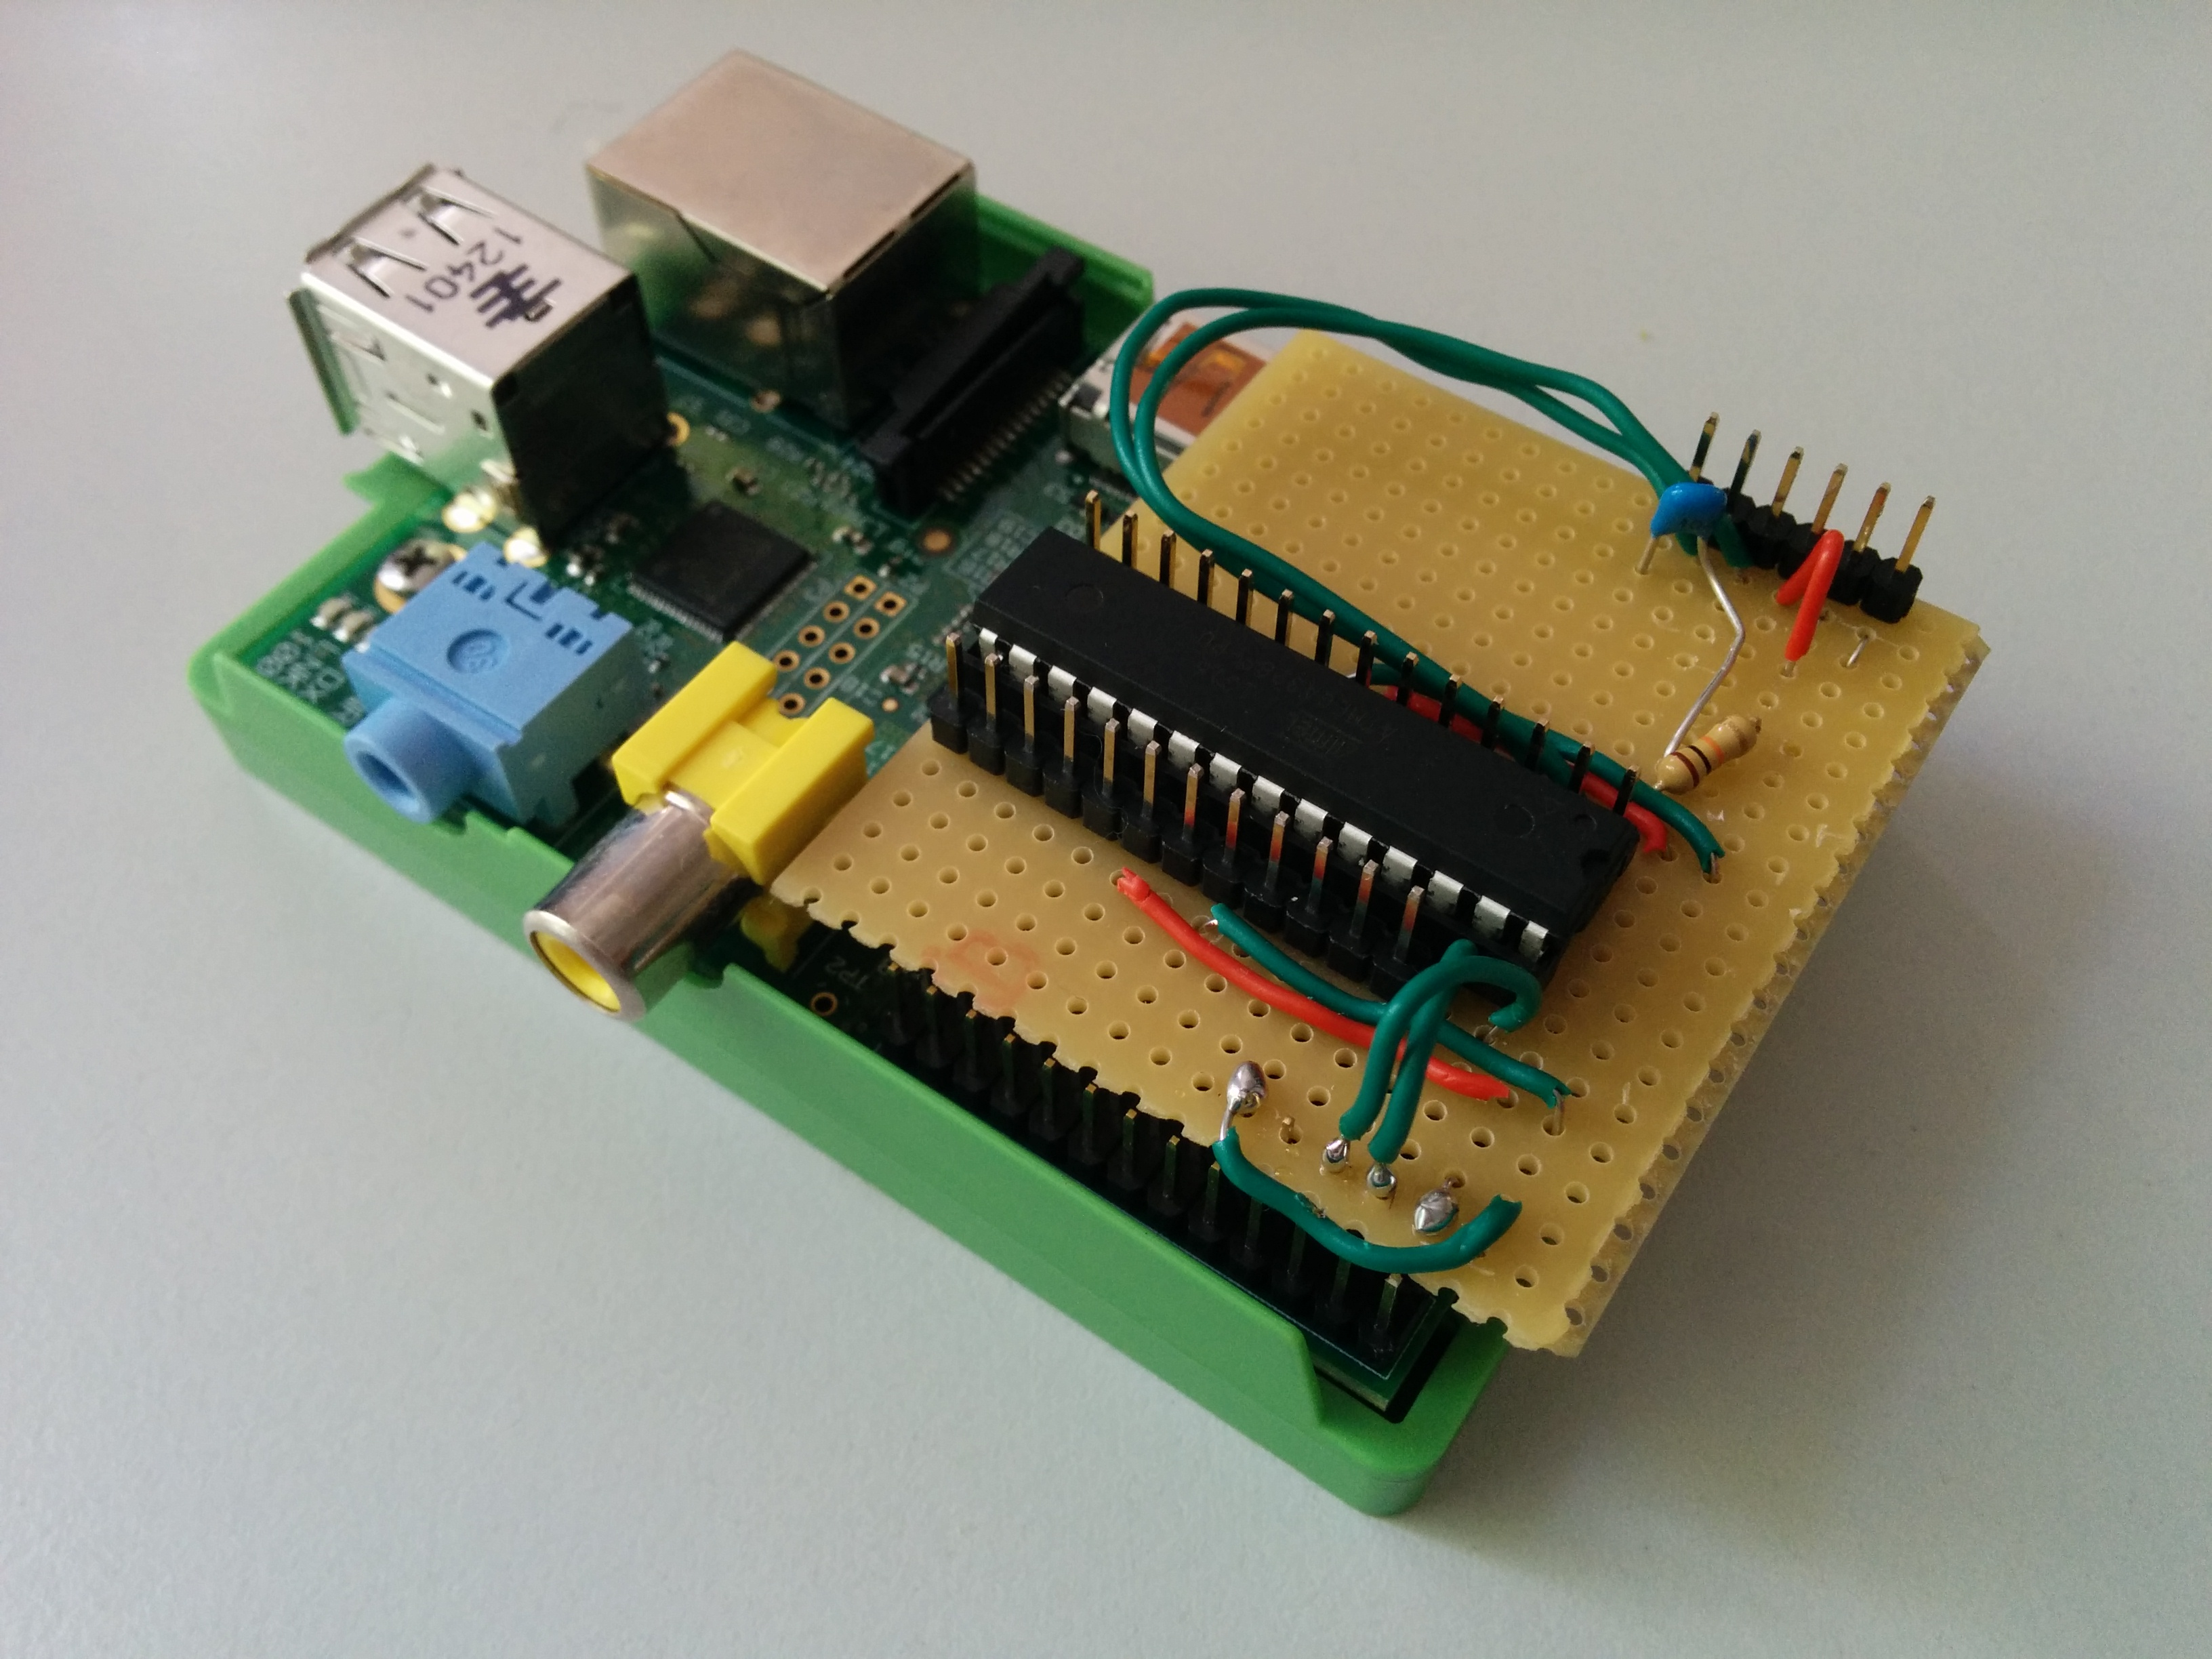
\includegraphics[width=10cm]{photos/IMG_20140623_144020.jpg}
  \end{center}
\end{frame}


\begin{frame}
\frametitle{Und wie geht das?}

\begin{itemize}
\item Nackter Atmega328P huckepack
\item Spannungsversorgung durch 3,3V-Schiene des Raspberry
\item Kommunikation �ber I2C-Bus - weitere Bus-Teilnehmer m�glich
\item \textbf{Bonus:} Atmega328P kann direkt vom Raspberry Pi programmiert werden
\end{itemize}
\end{frame}


\begin{frame}
\frametitle{Beispielcode Arduino}
  \begin{center}
    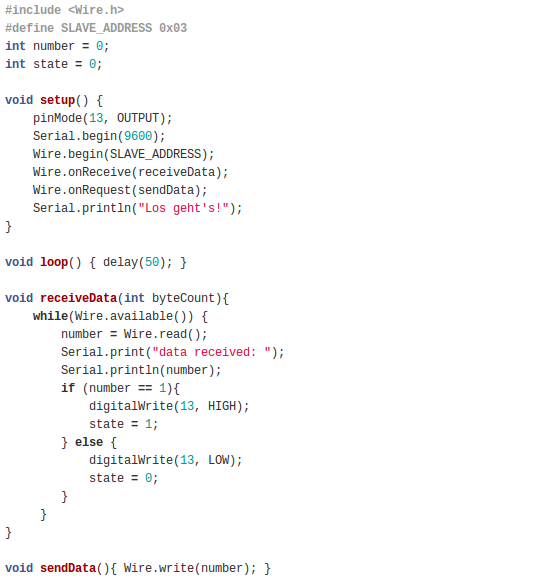
\includegraphics[width=6.3cm]{photos/i2carduino.png}
  \end{center}
\end{frame}

\begin{frame}
\frametitle{Beispielcode Raspberry}
  \begin{center}
    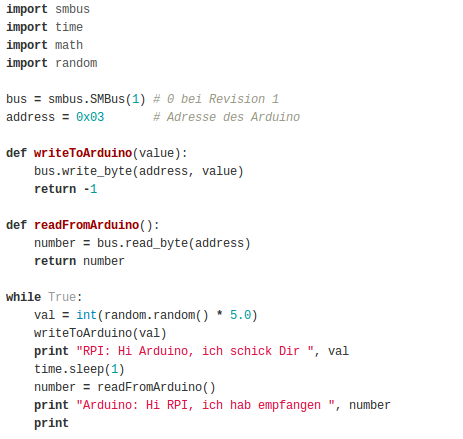
\includegraphics[width=6.3cm]{photos/i2craspberry.png}
  \end{center}
\end{frame}

\begin{frame}
\frametitle{Vor- und Nachteile}
\textbf{Vorteile}
\begin{itemize}
\item Billig: Atmega328P gibt es in der Fuzo beim blauen C
\item Schnell realisiert
\item Sehr flexibel
\end{itemize}

\textbf{Nachteile}
\begin{itemize}
\item Zwei Sprachen involviert: Python und Arduino
\item Kein fertiges Protokoll: Handarbeit angesagt
\item Nur bei 3,3V-Betrieb bleiben alle Vorteile von I\textsuperscript{2}C erhalten
\end{itemize}

\end{frame}

\subsection{Raspberry Pi als Zentrale}

\begin{frame} 
\frametitle{Kommunikation �ber's Netz}
Arduinos mit Enc28J60-Ethernetmodul kommunizieren mit dem Raspberry Pi:
\newline

\begin{itemize}
\item UDP-Kommunikation bei Arduino simpel realisierbar
\item UDP-Empfang auf Raspberry-Seite nur wenige Zeilen Python
\item Billige Hardware am Arduino (3 bis 5 \euro \ f�r Enc28J60) 
\item Weniger Einschr�nkungen bei Busl�nge gg�. direktem Onewire
\end{itemize}


\end{frame}